\chapter{A complete error propagation model}
\label{ch::model}
%
% Original title:
%   Modello del sistema di misura per triangolazione laser-telecamera e sua caratterizzazione
% In English:
%   A complete error propagation model for laser-camera triangulation systems
%
% Presentation to the chapter
  \textit{In this chapter we will present a complete mathematical model for errors propagation in \acs{SOL} systems, and discuss its characterization and limits. Furthermore we briefly present some alternative solutions analysed.}

% Problem definition
  \section{Problem definition}
Designing a new product is a very delicate process in which we have to consider all the details of interest. The purpose of this process is to maximise the final result. The greater is the product complexity, the more this process is tricky. In the case of study, a \acs{WPMS} is rated as good if the measures made with it are close enough to the real ones. A question rises: what does ``close enough'' mean? \\

As described in Chapter \ref{ch:technology}, a \acs{SOL} system is made up of many components: cameras, sensors, lenses, laser projectors, laser-camera reciprocal positions, etc. All of these components are sources of noise. Accurately control these sources, allows to significantly increase the accuracy of the output measurement. Unfortunately this is not only a problem of noise. When we design a new system we decide how to put the elements, how to link them and which positions are the best to reach our goal, but when too many elements are taken into account at the same time, it is very difficult to estimate the effect of each single choice on the final result. When there are no models or virtual system that allow to simulate this chain of effects, the only way to evaluate the quality of the system is to build and to try it on real situation or in laboratory, with a waste of time and money in the case the system doesn't reach given requirements. Time and money are two fundamental aspects in a company, specially when products have to be customized on customer needs, or when a new product have to be designed within a deadline. \\

By combining what has just been said with \acs{WPMS}s description in Chapter \ref{ch:sys_cmp}, both from the point of view of hardware and software, we can summarize the sources of noise/error for the acquisition of images and measurement, as follows:
  \begin{itemize}
    \item Environment
      \begin{itemize}
        \item Working tolerances
        \item Temperature range
        \item Installation
        \item Vibration/Shock
        \item External light conditions
        \item Dirty and wet condition on the target (wheel surface)
      \end{itemize}
      %
    \item Not ideal of the model
      \begin{itemize}
        \item Wheel yaw and camber
        \item Laser spot shape (discussed in Subsection \ref{subsec:lenses})
        \item Lenses (discussed in Subsection \ref{subsec:peak-detection})
      \end{itemize}
      %
    \item Images acquisition process
      \begin{itemize}
        \item Laser plane
        \item System calibration and geometrical parameters evaluation
        \item Profile extraction
      \end{itemize}
      %
    \item Data processing
      \begin{itemize}
        \item Point cloud interpolation
        \item Keypoints detection
        \item Measures evaluation and error propagation (Summaries and differences, application of closed formulas, \ldots)
      \end{itemize}
  \end{itemize}


The model proposed in this chapter aims to evaluate the error made determining a 3D point in the world, starting from the detection of its projection in the image. The model tries to consider all the elements described in Chapter \ref{ch:technology}, organizing them accordingly to the \acs{SOL} systems geometry. In particular, we will focus on the problem of sub-pixel point extraction. In the end, we will try to improve the model, considering the calibration problem and including the corrections due to the non-ideality of the image acquisition. \\

In Appendix \ref{ap:model} we summarized the proposed model, with particular attention to the notation and to the simplicity of comprehension. In Appendix \ref{ap:nomen} we added a table with all the definition of interests for this chapter.


% Introduction to error propagation
  \section{Introduction to error propagation}
Before studying the model, we briefly recall some notions on propagation of measurement errors. Accordingly with \cite{book:ivm}, the size is a property of an object that could be expressed by a number and a reference, i.e. it is measurable. Physical size measurement is generally followed by the error estimation associated with it, specially when they are indirect measure. In the general case, given the function $y = f(x)$, we can generalized its error as
  \begin{equation}
    \sigma_f = \begin{vmatrix}
      \frac{df}{dx}
    \end{vmatrix}_{x = x_0}
    \sigma_x
    \label{eq:er_prop_1}
  \end{equation}
If $y = f(\bar{x})$, function of $k$ variables, Equation \ref{eq:er_prop_1} can be generalize as:
  \begin{equation}
    \sigma_f = \sum_{j = 1}^k \begin{vmatrix}
      \frac{\partial f}{\partial x_j}
    \end{vmatrix}_{x = x_0}
    \sigma_x
    \label{eq:er_prop_2}
  \end{equation}
The propagation of the maximum errors by using the differential, is based on the assumption that infinitesimal variations of the variables are given by the respective errors. If we want to estimate the maximum error for $y$, it is appropriate to sum up all the terms consistently, i.e. taking the partial derivative modules.


% Triangulation system geometry
  \section{Triangulation system geometry}
\label{sec:init-modelanalysis}
At first, we analyse the errors due to the geometry of the triangulation system. For simplicity, we will focus on the standard geometry (described in Section \ref{sec:lctt}): the analysis for other geometries is trivial. \\

As illustrated in Figure \ref{fig:laser-triang}, the laser-camera pair form a triangle with angle $\phi$ between the baseline (the plane along the distance between the laser and the camera), and the optical axis of the camera. In \acs{SOL} systems, $\phi$ is
\clearpage
  \begin{figure}[h]
    \centering
    \begin{minipage}[c]{\textwidth}
      \centering
      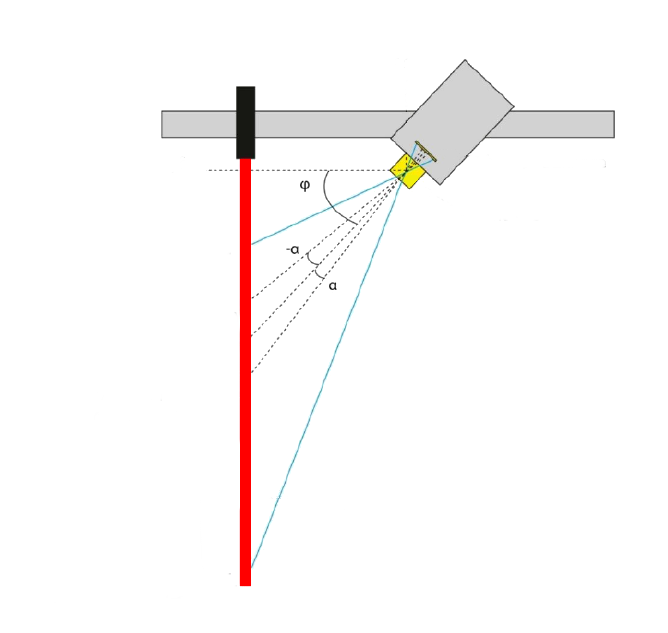
\includegraphics[width=0.7\textwidth]{./images/model/laser_triang.png}
      \caption{\acs{FOV} and characteristic angles}
      \label{fig:laser-triang}
    \end{minipage}
    \vfill
    \begin{minipage}[c]{\textwidth}
      \centering
      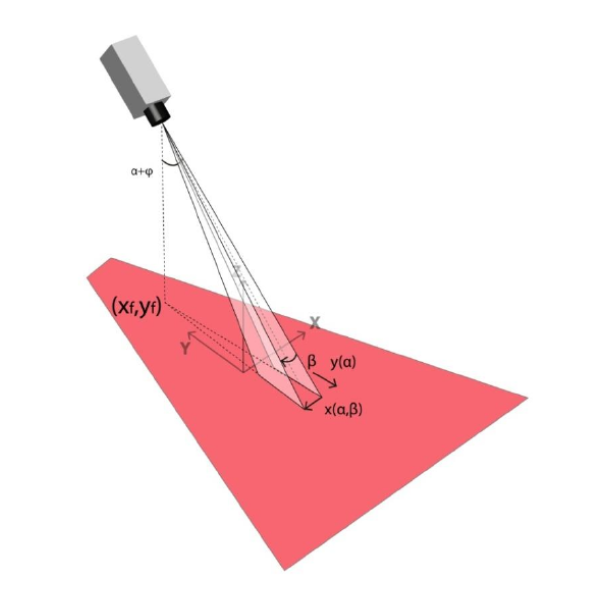
\includegraphics[width=0.7\textwidth]{./images/model/laser_triang_pdv.png}
      \caption{Angles definitions}
      \label{fig:laser-triang-pdv}
    \end{minipage}
  \end{figure}
\clearpage \noindent
called \textit{triangulation angle}. If $\phi$ and the baseline are known, any point in the 3D space belonging to the laser plane, is located estimating the offset $\alpha$ with respect to $\phi$, and the offset $\beta$ with respect to the optical axis of the camera. Accordingly with \cite{th:quattrini}, and using simple mathematical relations, we can locate the $y$ coordinate as function of the angle $\alpha$ as follows:
  \begin{equation}
    \label{eq:model-ya}
    y\left( \alpha \right) = y_f + z_f \tan \left( \phi + \alpha \right)
  \end{equation}
where $\left( x_f, y_f, z_f \right)$ are the principal point projection coordinates in the laser plane (in the world reference system), as shown in Figure \ref{fig:laser-triang-pdv}. Note that using this notation, $z_f$ is the distance from the laser to the camera, previously called baseline. \\

Now let's look at the Figure \ref{fig:laser-triang-pdv}. As mentioned at the end of the Section \ref{sec:lctt}, camera's resolutions varies changing the distance of the target from the camera. In particular this is true for the resolution along the laser line (axis $x$ with respect to out notation). Points having the same $x$ coordinates but different $y$ are estimated with different camera resolutions. This means that the values of $x$ strongly depends on the angle $\beta$ (that identify the value of $x$ with respect the the optical axis of the camera), but also on the angle $\alpha$ (that identifies the value of $y$ with respect to the triangulation angle). For these reasons we can write
  \begin{equation}
  \label{eq:model-xab}
    x(\alpha, \beta) = \frac{y\left( \alpha \right) - y_f}{\sin(\phi + \alpha)}\tan(\beta)
  \end{equation} \\
As we can see, $x$ strongly depends on $y$, accordingly with what we said in Section \ref{sec:lctt}, about the trapezoidal shape of the laser plane. Still for the shape of the laser, a similar consideration can be made for the $y$ coordinate, because of the trapezoidal shape of the laser plane.
% To be precise, a similar consideration can be made for the $y$ coordinate, because of the trapezoidal shape of the laser plane.
However, in this case the differences between the nearest and the farthest \acs{FOV}s along the $x$ axis, are negligible. For theses reasons we will consider Equation \ref{eq:model-ya} as a good approximation of the relation between $y$ and $\alpha$. \\

Accordingly with what we said in Section \ref{sec:teo-calibration}, during calibration phase the choice of the reference system is arbitrary, so we can put $\left( x_f, y_f, z_f \right) = \left( 0, 0, z_f \right)$ without loss of generality. In this way, Equations \ref{eq:model-ya} and \ref{eq:model-xab} can be simplified. \\

At this point it is easy to estimate the error associated with the two newly introduced measures. Applying the simplification, for Equation \ref{eq:model-ya} we can write:
  \begin{equation}
    \label{eq:model-ya-err0}
    \sigma_{y_\alpha} = \sqrt{
      \left( \frac{\partial y}{\partial z_f} \right)^2 \sigma_{z_f}^2 +
      \left( \frac{\partial y}{\partial \phi} \right)^2 \sigma_\phi^2 +
      \left( \frac{\partial y}{\partial \alpha} \right)^2 \sigma_\alpha^2
    }
  \end{equation}
while for Equation \ref{eq:model-xab} we can write
  \begin{equation}
    \label{eq:model-xab-err0}
    \sigma_{x\left( \alpha, \beta \right)} = \sqrt{
      \left( \frac{\partial x}{\partial \phi} \right)^2 \sigma_\phi^2 +
      \left( \frac{\partial x}{\partial \alpha} \right)^2 \sigma_\alpha^2 +
      \left( \frac{\partial x}{\partial \beta} \right)^2 \sigma_\beta^2
    }
  \end{equation}\\
In these last equations, the $\sigma$ are the errors committed evaluating each component in the Equations \ref{eq:model-ya} and \ref{eq:model-xab}. As we can see, in Equations \ref{eq:model-ya-err0} and \ref{eq:model-xab-err0} we are considering also $\phi$ and $z_f$ that are constructive parameters that depend on the accuracy with which the system was built or installed. Typically, these parameters are corrected thanks to the calibration process, that allows to estimate camera intrinsic and extrinsic parameters, as mentioned in Section \ref{sec:teo-calibration}. In addition, the calibration process uses many algorithms that in turn use different heuristics to estimate camera parameters. This means that all parameters are affected by error, but as we can see later, we can consider these errors negligible. So we can simplify Equations \ref{eq:model-ya-err0} and \ref{eq:model-xab-err0} respectively as follows
  \begin{equation}
    \label{eq:model-ya-err1}
    \sigma_{y_\alpha} = \sqrt{
      \left( \frac{\partial y}{\partial \alpha} \right)^2 \sigma_\alpha^2
    }
  \end{equation}
  
  \begin{equation}
    \label{eq:model-xab-err1}
    \sigma_{x\left( \alpha, \beta \right)} = \sqrt{
      \left( \frac{\partial x}{\partial y_\alpha} \right)^2 \sigma_{y_\alpha}^2 +
      \left( \frac{\partial x}{\partial \alpha} \right)^2 \sigma_\alpha^2 +
      \left( \frac{\partial x}{\partial \beta} \right)^2 \sigma_\beta^2
    }
  \end{equation} \\

Keeping focus on the geometry of the system, the second element to consider is the laser plane. In standard geometry, variations on laser pitch and roll rotations, with respect to the reference system, can affect heavily the final measure. By trigonometry we know that by changing the angle, the point projections also change in the two axes of the reference system. The same effect is present when we rotate the laser plane with respect to the $x$ axis (roll) or with respect to the $y$ axis (pitch). These errors are more apparent in the other triangulation geometries. What we have to do, is to compensate these rotations projecting the laser plane on the ideal one. The compensations are performed as follows:
  \begin{equation}
    \begin{matrix}
      y_w = y(\alpha) \cdot cos(\rho) \\ ~ \\
      x_w = x(\alpha, \beta) \cdot \cos(\gamma)
    \end{matrix}
    \label{eq:radial-compensations}
  \end{equation} \\
where $\rho$ is the laser roll angle, and $\gamma$ is the laser pitch angle. Using the model introduced in Equation \ref{eq:er_prop_2}, we can write, respectively:
  \begin{equation}
    \sigma_{y_w} = \sqrt{
      \left( \frac{\partial y_w}{\partial y(\alpha)} \right)^2 \sigma_{y_\alpha}^2
      + \left( \frac{\partial y_w}{\partial \rho} \right)^2 \sigma_\rho^2
    }
    \label{eq:err-radial-comp-yw}
  \end{equation}
  \begin{equation}
    \sigma_{x_w} = \sqrt{
      \left( \frac{\partial x_w}{\partial x\left( \alpha, \beta \right)} \right)^2 \sigma_{x\left( \alpha, \beta \right)}^2 +
      \left( \frac{\partial x_w}{\partial \gamma} \right)^2 \sigma_\gamma^2
    }
    \label{eq:err-radial-comp-xw}
  \end{equation} \\
where $\sigma_{y_\alpha}$ and $\sigma_{x\left( \alpha, \beta \right)}$ are the ones evaluated in Equations \ref{eq:model-ya-err1} and \ref{eq:model-xab-err1} respectively. \\

A practical example in which these compensations are needed, is the \acs{WPMS}. In autonomous \acs{WPMS}s placed alongside the rails, specular geometry is generally used, and wheels are measured while the train is running. In these cases we are not sure to measure the wheel exactly along its axis, so the acquired profiles have to be compensated. This type of correction is called \textit{radial compensation}. \\
% The errors due to non-ideality of laser plane placement can be seen also as non-ideality of work conditions. In autonomous \acs{WPMS}s placed alongside the rails, specular geometry is generally used, and wheels are measured while the train is running. In these cases we are not sure to measure the wheel exactly along its axis, and typically corrections like the ones for rolls are needed. In these field, these corrections are referred as \textit{radial compensation}. \\
We can consider the same things about pitch. Sometimes the wheel under analysis is not perpendicular with the laser plane, because wheel yaw and camber. Also in these cases $x$ values must be compensated.

%We can see here, the determination of $x$ is fully dependent by the formulation on $y$.


% Word to camera discretization
  \section{World to image plane}
\label{sec:wrd2cam}
Accordingly with what we reported in Section \ref{sec:pinhole_camera}, the second step is to determine the 3D point coordinates in a reference system concordant with the image plane. The plane of interest $S$ is a plane parallel with lens plane and passing through the plane parallel to the sensor.  This choice is due to the possibility to tilt the lens with respect to the sensor, accordingly with the Scheimpflug principle, described above. If we consider the image plane parallel to the sensor directly, some issue arises. Tilting the lens changes the focal length of the camera, that varies point by point, resulting in a distorted image. This problem can be simplified observing that if we tilt the lens, we add an image plane rotated with respect to the classical image plane. In this way, the transformation between the two planes is a simple projection between planes. So we decided to split the problem in two subproblems: the first, described in this section, requires to change coordinates reference system; the second, described in Section \ref{sec:scheimflug}, needs to project the point on a different plane. Furthermore, this choice allows to simplify the mathematical model. \\

Let's focus on the Figure \ref{fig:laser-triang-a}.
  \begin{figure}[t!]
    \centering
    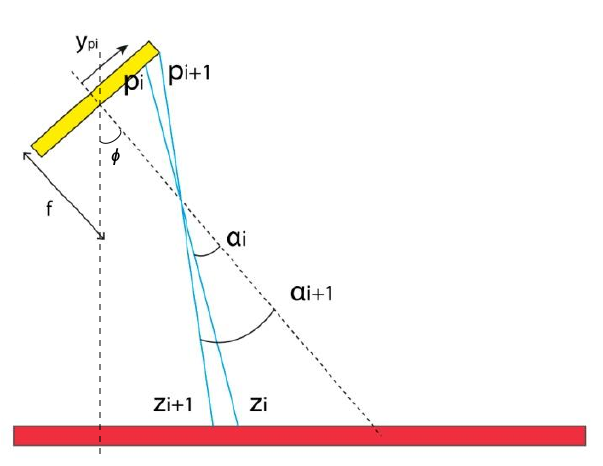
\includegraphics[width=0.7\textwidth]{./images/model/laser_triang_alpha.png}
    \caption{World to image plane}
    \label{fig:laser-triang-a}
  \end{figure}
As we can see, a change in the 3D point coordinates causes a variation in the image plane. However this alterations deals with the angle $\alpha$, estimated as offset from the triangulation angle $\phi$. Furthermore, laser plane and image plane are not parallel: this means that the two variations are different. What we are interested in, is the variation on the image plane, not in the world, so we can formulate this problem, accordingly with \cite{th:quattrini}, as:
  \begin{equation}
  	\alpha_i = \arctan\left( \frac{y_{s_i}}{f} \right)
    \label{eq:model:alpha}
  \end{equation}
where $y_{s_i}$ is the $i^{th}$ points in the image plane $S$. Being careful, it is simple to observe that the same relation is valid when determining the error due evaluating the $x$ coordinate, but with respect to the optical axis:
  \begin{equation*}
  	\beta_i = \arctan\left( \frac{x_{s_i}}{f} \right)
  \end{equation*}
Note that this step is important also to determine the natural camera resolution, in fact it allows to define the minimum variation appreciated by the sensor while it is observing the world.

So we can conclude writing that:
  \begin{equation}
    \label{eq:det_a}
  	\sigma_{\alpha_i} = \sqrt{
  	  \left( \frac{\partial \alpha_i}{\partial y_{s_i}} \right)^2 \sigma_{y_{s_i}}^2
  	  + \left( \frac{\partial \alpha_i}{\partial f} \right)^2 \sigma_f^2
  	}
  \end{equation} \\

Also in this case, $f$ is a parameter estimated thanks to the calibration processes, so we can consider it as negligible. Then, we can simplify Equation \ref{eq:det_a} as
  \begin{equation*}
  	\sigma_{\alpha_i} = \sqrt{
  	  \left( \frac{\partial \alpha_i}{\partial y_{s_i}} \right)^2 \sigma_{y_{s_i}}^2
  	}
  \end{equation*}
The same conclusions can be applied to $\beta_i$. \\

As we will see later, this transformation is the most delicate one, probably because of the change of reference system. In fact we can consider it as a passage from 3D to 2D reference system.


% Scheimpflug geometry
  \section{Scheimpflug geometry}
\label{sec:scheimflug}
As introduced in the previous section, now, we describe the plane correction due to the application of Scheimpflug principle, tilting the lens. \\

Tilting lenses causes a variation of the image plane, which rotates to stay parallel to the lens itself. Many works, such as \cite{inproc-lens-inc}\cite{Louhichi2006}\cite{4059344}, tried to improve the calibration processes, introducing different corrections in order to balance the effects introduced by lens tilt. For the most part, they have tried to apply different rotations to the plane, but these have been shown to work only for small angles. For big angles, the rotations are not enough. \\

Consider the two image planes, the one parallel to the sensor and the tilted one: as shown in Figure \ref{fig:scheimpflug-line}, the origin of the two planes is the same, since the parallel plane can be arbitrarily placed.
  \begin{figure}[t!]
    \centering
    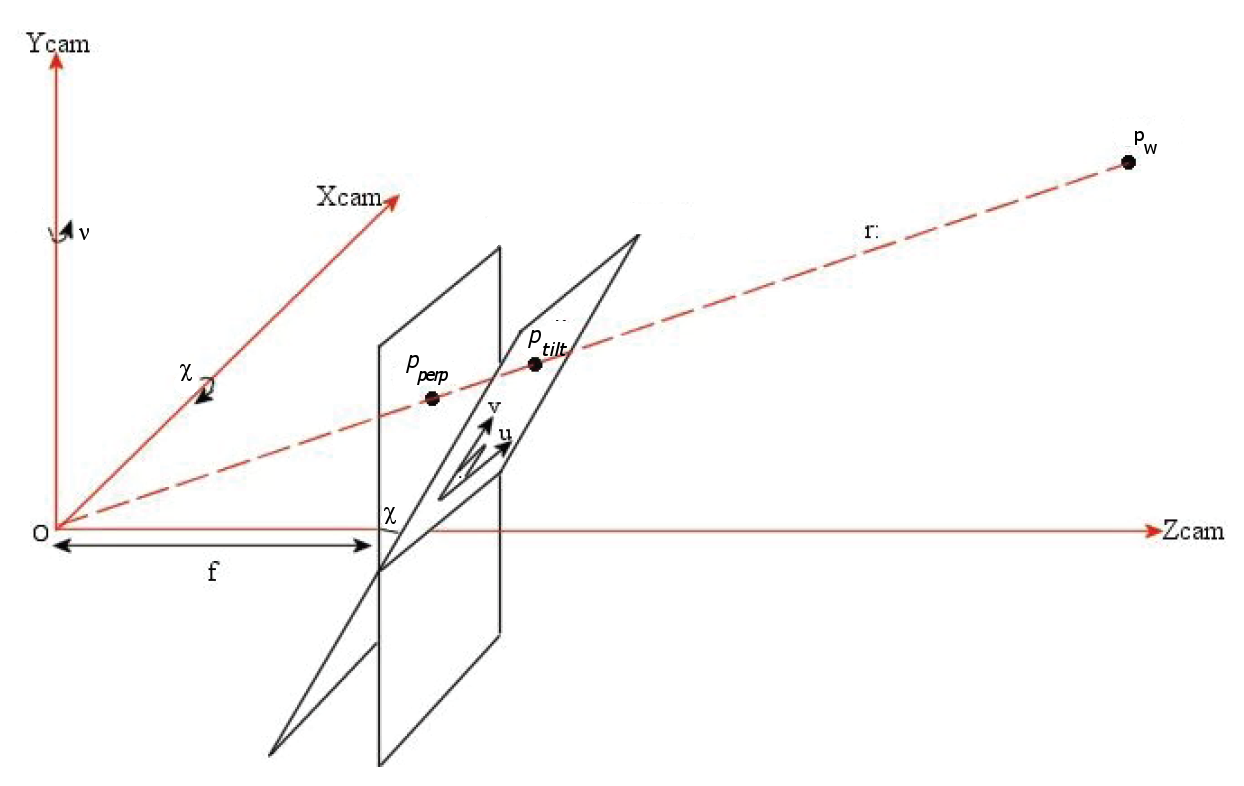
\includegraphics[width=\textwidth]{./images/model/scheimpflug.png}
    \caption{Intersection of the point in the real world in the tilted plane and in the perpendicular plane.}
    \label{fig:scheimpflug-line}
  \end{figure}
Similar to what is shown in the Figure \ref{fig:perspective_projection}, we can draw a line $r$ from the optical center $O$ to the point $p_w = \left( x_w, y_w, z_w \right)$ in the world. Accordingly with the sections above, $p_w$ is a point belonging to the laser plane, without considering radial compensation, and the tilted plane is the one in which we have projected $p_w$ in Section \ref{sec:wrd2cam}. Accordingly with \cite{SchCameraCalib}, the line $r$ passes through the two planes, allowing the definition of a system of equations that solve the intersection problem. The solution of this system can be written as follows:

  \begin{equation*}
      x_p = \lambda \cdot \left( x_s \cdot \cos\chi + y_s \cdot \sin\upsilon\cos\chi \right)
  \end{equation*}
  \begin{equation*}
    y_p = \lambda \cdot y_s \cdot \cos\upsilon
  \end{equation*}
where $\left( x_p, y_p\right) = p_{perp}$ in the figure, and $\left( x_s, y_s\right)$ ($p_{tilt}$ in figure) are the coordinate of the point in the sensor reference system, introduced in the section above. The parameter $\lambda$ is the plane coefficient and it is:
  \begin{equation*}
    \lambda = \frac{f}{f + x_s \sin\chi + y_s \sin\upsilon\cos\chi}
  \end{equation*}
The angles $\chi$ and $\upsilon$ are the swing and tilt angle of the lens, respectively. In literature, the term swing refers to a rotation with respect to the $x$ axis, while tilt refers to a rotation with respect to the $y$ axis. \\

The equation considered has been defined in a proposal for an algorithm for camera calibration. Despite that, the model capability to consider point projections gives to it a big advantage over simple rotations: the fact that we are able to consider also perspective distortions, as we have done in Section \ref{sec:pinhole_camera} for world to camera coordinate systems transformations. Note that also in this case, the $x$ coordinates are function of the $y$ ones. \\

From an analytical point of view, this is the most delicate step. The big number of elements to consider makes this calculation a big source of error. The error propagation model suggests to compute

  \begin{equation*}
    \sigma_{x_{s_i}} = \sqrt{
      \left( \frac{\partial x_{s_i}}{\partial y_{p_i}} \right)^2 \sigma_{y_{p_i}}^2 +
      \left( \frac{\partial x_{s_i}}{\partial x_{p_i}} \right)^2 \sigma_{x_{p_i}}^2 +
      \left( \frac{\partial x_{s_i}}{\partial \upsilon} \right)^2 \sigma_\upsilon^2 +
      \left( \frac{\partial x_{s_i}}{\partial \chi} \right)^2 \sigma_\chi^2
    }
  \end{equation*}
  \begin{equation*}
    \sigma_{y_{s_i}} = \sqrt{
      \left( \frac{\partial y_{s_i}}{\partial y_{p_i}} \right)^2 \sigma_{y_{p_i}}^2 +
      \left( \frac{\partial y_{s_i}}{\partial x_{p_i}} \right)^2 \sigma_{x_{p_i}}^2 +
      \left( \frac{\partial y_{s_i}}{\partial \upsilon} \right)^2 \sigma_\upsilon^2 +
      \left( \frac{\partial y_{s_i}}{\partial \chi} \right)^2 \sigma_\chi^2
    }
  \end{equation*} \\
  
\noindent
Even in this case we could ignore the contribution of the focal length, because it is a parameter estimated by the calibration process.\\

To complete this model, we should take into account also focal length and image center transformations. Reference \cite{SchCameraCalib} suggests the following set of relations:
  \begin{equation*}
    f' = \frac{f}{\cos\upsilon}
  \end{equation*}
  \begin{equation*}
    C_x' = C_x + f\cdot n_x \cdot \sin\upsilon
  \end{equation*}
  \begin{equation*}
    C_y' = C_y + f\cdot n_y \cdot \sin\chi
  \end{equation*} \\
However, our tests (described below) demonstrated that these corrections are useless. Calibration algorithms that do not implement this type of heuristics, will implement parameters (i.e focal length and optical center) optimization methods anyway, that try to evaluate these parameters as precisely as possible. The methods seem to be accurate enough to ignore the latter passages, in favour of ones suggested by the calibration.


% Lens distortion
  \section{Lens distortion and point discretization}
\label{sec:model-lens-distortion}
In Section \ref{subsec:lenses} we have introduced lenses, highlighting their advantages over the pinhole. We also introduced the differences between the thin lens model and the thick lens one, observing how, in both cases, curvature radii could introduce aberrations on the acquired image.

As we said in Section \ref{sec:teo-calibration}, all the calibration algorithms try to solve this problem, but most of them, like Tsai and Zhang, are limited to considering radial distortions. In fact it can be shown that tangential contributions are typically negligible, while radial ones increase when focal length decreases. Fortunately, in literature there are some studies about lenses and thin prism distortions, such as \cite{brown},\cite{DBLP:journals/corr/cs-CV-0308003} and \cite{Heikkila}, which offer some solutions to extend the analysis beyond this limit. \\

As a first thing, we focused on \cite{TsaiTvLenses}. Accordingly with it, the commonly used polynomial for radial distortion model, is given by the series
  \begin{equation}
    \label{eq:radial-tot}
    r_d = r + \delta_r = r + \sum_{j=1}^\infty k_jr^{(2j)}
  \end{equation}
where $r$ is the lens radius and $k_j$ is the radial coefficient of degree $j$. As we will discuss later, the used calibration algorithm are limited to the second order, so Equation \ref{eq:radial-tot} can be reduced as:
  \begin{equation}
    \label{eq:radial-2}
    r_d = r + k_1r^2 + k_2r^4
  \end{equation}

Applying Equation \ref{eq:radial-2} to distorted points, we found a simple relation, similar to that in \cite{TsaiTvLenses}:
  \begin{equation}
    \label{eq:dist-coords}
    x_{p_i} = x_{p_i}^{d} \left( 1 + k_1r^2 \right) \qquad
    y_{p_i} = y_{p_i}^{d} \left( 1 + k_1r^2 \right)
  \end{equation}
where $\left( x_{p_i}^{d}, y_{p_i}^{d} \right)$ are the distorted coordinates in the parallel to sensor image plane. In this way, we can determine the projection of a 3D point in a plane parallel to the sensor and distortion free. Note that, given a specific point, it does not make sense to consider the whole radius $r$ of the lens, so it is preferable to consider its distance from the point to the optical center (that ideally is locate in the center of the lens). \\
As we have done in previous sections, the error is propagated as follows
  \begin{equation}
    \label{eq:sigma-dist}
    \begin{matrix}
      \sigma_{x_{p_i}} = \sqrt{
        \left( \frac{\partial x_{p_i}}{\partial x_{p_i}^d} \right)^2 \sigma_{x_{p_i}^d}^2
        + \left( \frac{\partial x_{p_i}}{\partial k_1} \right)^2 \sigma_{k_1}^2
      }
      \\~\\
      \sigma_{y_{p_i}} = \sqrt{
        \left( \frac{\partial y_{p_i}}{\partial y_{p_i}^d} \right)^2 \sigma_{y_{p_i}^d}^2
        + \left( \frac{\partial y_{p_i}}{\partial k_1} \right)^2 \sigma_{k_1}^2
      } 
    \end{matrix}
  \end{equation}
Note that this transformation is the same for both $x$ and $y$, thanks to lens radial distortion symmetry. \\

At this point we have noticed that it is very easy to spread the solution to the tangential distortions. Accordingly with \cite{Heikkila} we observed that Equations \ref{eq:radial-2} could be extended easily:
  \begin{equation*}
    \mathcal{F}\left( r, \bar{k}, \bar{p} \right) = 
    \begin{bmatrix}
      x_{p_i}\left( \sum_{j=1}^\infty k_jr^{2j} \right) + \left( 2 p_1 x_{p_i} y_{p_i} + p_2 \left( r^2 + 2 x_{p_i}^2  \right) \right) \left( 1 + p_3 r^2 + \ldots  \right)
      \\
      y_{p_i}\left( \sum_{j=1}^\infty k_jr^{2j} \right) + \left(  p_1 \left( r^2 + 2 y_{p_i}^2  \right) + 2 p_2 x_{p_i} y_{p_i} \right) \left( 1 + p_3 r^2 + \ldots \right)
    \end{bmatrix}
  \end{equation*}
As we can see, to consider tangential distortion some additive factors are needed. The analysis for error propagation is the same as that for the Equation \ref{eq:sigma-dist}, but we have to pay attention to include the partial derivatives of the tangential coefficients. \\
To complete the analysis, we have done some test using nominal lens parameters given by the manufacturer, and we observed that the error improvement was negligible. \\

In the last two cases we could ignore the components depending by distortion coefficients, that we can consider correct thanks to calibration processes. \\

Looking around, we have found another model that we considered of interest. Accordingly with \cite{DBLP:journals/corr/cs-CV-0308003}, radial distortions could be formulated as a rational distribution like:
  \begin{equation*}
    \mathcal{F}\left( r, \bar{k}, \bar{p} \right) = \frac{1 + k_1r + k_2r^2}{1 + k_3r + k_4r^2 + k_5r^3}
  \end{equation*}
It is easy to derive many other formulas from the general one, and the most interesting are shown in Table \ref{tab:dist-funcs}.
  \begin{table}[t!]
  \centering
  \begin{tabular}{r|l}
  \multicolumn{1}{c|}{\textbf{\#}} & \multicolumn{1}{c}{\textbf{$\mathcal{F}\left( r, \bar{k} \right)$}} \\
    \hline
    1	& $1 + k_1 r$ \\
    2	& $1 + k_1 r^2$ \\
    3	& $1 + k_1 r + k_2 r^2$ \\
    4	& $1 + k_1 r^2 + k_2 r^4$ \\
    5	& $1 / (1 + k_1 r) $ \\
    6	& $1 / (1 + k_1 r^2)$ \\
    7	& $(1 + k_1 r) / (1 + k_2 r^2)$ \\
    8	& $1 / (1 + k_1 r + k_2 r^2)$ \\
    9	& $(1 + k_1 r) / (1 + k_2 r + k_3 r^2)$ \\
    10	& $(1 + k_1 r^2) / (1 + k_2 r + k_3 r^2)$ \\
    \hline
  \end{tabular}
  
  \caption{Polynomial and rational distortion functions}
  \label{tab:dist-funcs}
\end{table}
All these functions enjoy some properties,. in fact they are:
  \begin{itemize}
    \item radially symmetric around the center of distortion;
    \item expressed in terms of the radius $r$ only;
    \item continuous and $r_d = 0$ iff $r = 0$;
    \item the approximation of $x_d$ is an odd function of $x$.
  \end{itemize}
The above three properties act as the criteria to be good candidates as radial distribution functions. Despite that, we can see that Equation \#4 is very closed to the Equation \ref{eq:radial-2}. Furthermore, the calibration algorithms we have used are limited to second degree, and in this conditions many of these equations can be traced back to \#4. At the end, it can be shown that the performances of the remaining functions are comparable with \#4. \\
For all these reasons, we focused only on Equations \ref{eq:dist-coords}, but as we have shown in this section, it is easy to extends it to tangential distortion or to increase its degree.

\bigskip
Once we have determined the distorted point in the image plane, the last step is the point discretization. In this phase we are interested in projecting the undistorted point in the distorted sensor plane. Accordingly with \cite{TsaiTvLenses}, this projection can be performed by centering the coordinate reference system in the optical center estimated during calibration processes, and by normalizing the point value in the sensor pixel range. At the end we can write:
  \begin{equation*}
    x_{p_i}^d = d_x'(x_{c_i} - c_x) \qquad \qquad y_{p_i}^d = d_y'(y_{c_i} - c_y)
    % \label{eq:discrete-coords}
  \end{equation*} \\
where $(c_x, c_y)$ is the optical center, and $(d_x', d_y')$ the normalized pixel center to center distance, along $x$ and $y$ axis, respectively. Consistent with what we have done so far, we can conclude with error propagation:
  \begin{equation}
    \begin{matrix}
    %
    \sigma_{x_{p_i}^d} = \sqrt{
      \left( \frac{\partial x_{p_i}^d}{\partial x_{c_i}} \right)^2 \sigma_{x_{c_i}}^2
      + \left( \frac{\partial x_{p_i}^d}{\partial c_x} \right)^2 \sigma_{c_x}^2
    }
  %\end{equation*}
  \\
  %\begin{equation*}
    \sigma_{y_{p_i}^d} = \sqrt{
      \left( \frac{\partial y_{p_i}^d}{\partial y_{c_i}} \right)^2 \sigma_{y_{c_i}}^2
      + \left( \frac{\partial y_{p_i}^d}{\partial c_y} \right)^2 \sigma_{c_y}^2
    }
    %
    \end{matrix}
    \label{eq:model:err:disc}
  \end{equation} \\

\bigskip
Before concluding this section, we want to emphasize a possible source of ambiguity in understanding this model. The explanation started from the end of the chain and follows until the beginning. This choice was taken to better identify, for each step, the elements to analyse, and from which each relation depends. In this way the error determination was easy. However, we have to notice that we want to determine the error committed evaluating the point in the world, starting from pixel detection in the image, then formulas have to interpret in this sense, from pixel to world.

  
% Laser peaks detection
  \section{Laser peaks detection}
\label{sec:laser-peaks}

Starting from the point $ p_w = \left( x_w, y_w, z_w \right)$ in the 3D space, we reached its projection $p_c = \left( x_c, y_c \right)$ in the sensor reference system. At this point, the error committed while locating the peak, now depends by the technique used. \\

If we consider the general case, without using any sub-pixel approximation, the peak will be consider in the center of the pixel, i.e. located in $p_c$. Accordingly with \cite{th:quattrini}, we can model the distribution of all the possible positions of the peak along a specific direction as a \textit{uniform distribution}, centered in $p_c$, thus we can evaluate the location error with the standard deviation of the distribution, that is
  \begin{equation*}
    \sigma_{p_c} = \sqrt{\frac{\left(b - a\right)^2}{12}}
  \end{equation*}
with $a$ and $b$ the extremes of the range. \\
Let's consider the laser in its coordinates reference system. The use of a line lens allows us to spread the spot energy along a line. From a physical point of view, the signal we obtained in this way, is continuous along the direction of the abscissa, while from a mathematical point of view, the laser can be modelled as a solid Gaussian, like the one shown in Figure \ref{fig:mod-laser-line}.
  \begin{figure}[t!]
    \centering
    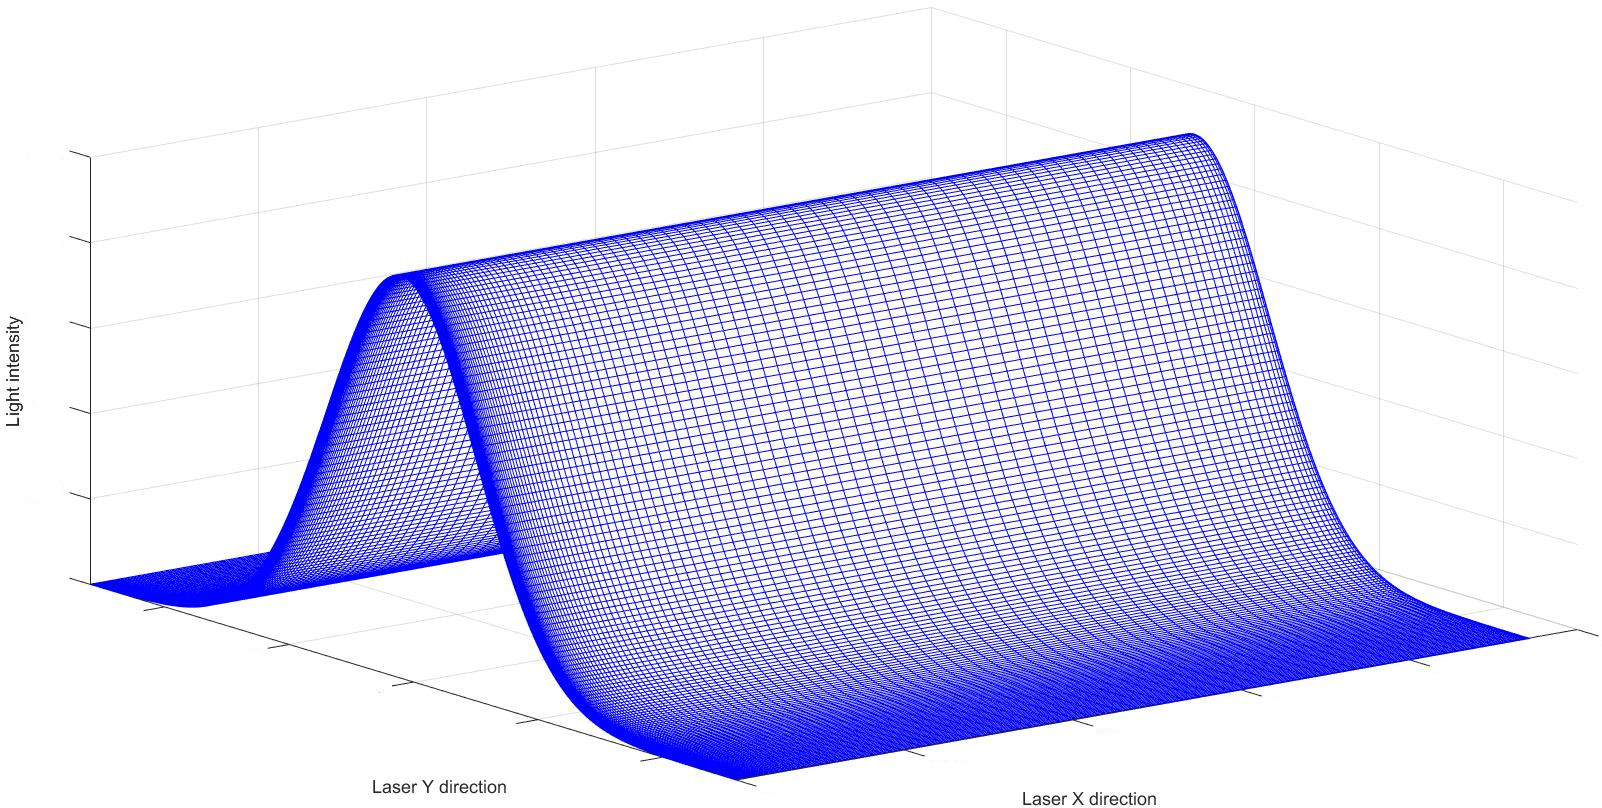
\includegraphics[width=0.8\textwidth]{./images/model/3Dgauss_grid.jpg}
    \caption{3D model of the laser line}
    \label{fig:mod-laser-line}
  \end{figure}
As we can see, we haven't any information about the position of the laser spot along the abscissa, so the only way to estimate the committed error is to use the distribution above. Thus, we modelled our error as follows:
  \begin{equation*}
    \sigma_{x_{c_i}} = \sqrt{\frac{\left(pixel \,\, size \right)^2}{12}}
  \end{equation*}
where the $pixel \,\, size$ is the ideal size of the pixel (along the $x$ axis if we assume it rectangular shaped). \\

A similar analysis can be made along the ordinate. However, even in conditions like the one shown in Figure \ref{fig:mod-laser-line}, along the ordinate we have always some informations about the shape of the laser line. This suggested us that it should be possible to consider all the mathematical models discussed in Subsection \ref{subsec:peak-detection}. In this way we should improve the detection of the laser spot peak, reducing the initial error. \\
In \cite{Naidu1991}, the authors present an interesting study on the precision of the approximations that we have considered above, nevertheless we are not convinced of the results they have achieved:
  \begin{itemize}
    \item First of all, we think that some of the proposed forms of $\hat{\delta}$ are incorrect. To validate our hypothesis, we evaluated from scratch each proposed filters. We reported our result in Table \ref{tab:local-mod}. As we can see, in particular for what concerns the approximation thought by Blaise and Rioux, the proposed model is too simplified. Short tests shown that the simplification made by \cite{Naidu1991} are too strong to be negligible, and from our point of view, they could be a source of errors. Furthermore, proposed results was estimated using a first-order approximation of the Gaussian, which further simplifies the problem. In short, we concluded that the problems are more complex than the paper shown.
    \item For each proposed model, the authors introduce a different constant, called $\alpha$, that allows to improve arbitrarily the filters performance. We noticed that they don't explain how they reached their results, and it seems that the value of $\alpha$ changes if we change the width of the laser spot: from a design point of view this is not acceptable.
    \item The proposed results were evaluated only in a specific condition (laser $\sigma \in \begin{bmatrix} 0.5 & 1 & 1.5 \end{bmatrix}$), which seems to be out of the actual working conditions.
  \end{itemize}
Hence, we decided to pass over suggested evaluations, and we looked for an alternative solution. \\
  \begin{table}[t!]
  \centering
  \begin{tabular}{|ccc|}

  \hline
  \textbf{Estimator}          & \textbf{Window} & \textbf{Local Estimator} \\
  \hline
  & & \\
  \textit{Gaussian}           & 3               &  $\delta$                \\ 
  & & \\ % \hline
  \textit{Linear}             & 3               & $\frac{\delta}{\sigma^2} \frac{e^{-\frac{1}{2\sigma^2}}}{1 - \left( 1 - \frac{\delta}{\sigma^2} \right) e^{-\frac{1}{2\sigma^2}}}$ \\ 
  & & \\ % \hline
  \textit{Parabolic}          & 3               & $\frac{\delta}{2\sigma^2} \frac{e^{-\frac{1}{2\sigma^2}}}{1-e^{-\frac{1}{2\sigma^2}}}$ \\ 
  & & \\ % \hline
  \textit{Center of Mass}     & 3               & $ \frac{2\delta}{\sigma^2} \frac{ e^{-\frac{1}{2\sigma^2}} }
                                                                         {  1+2e^{-\frac{1}{2\sigma^2}} }$ \\ 
  & & \\ % \hline
  \textit{Center of Mass}     & 5               & $ \frac{2\delta}{\sigma^2} \frac{ e^{-\frac{1}{2\sigma^2}} + 4e^{-\frac{4}{2\sigma^2}} }
                                                                         {1 + 2e^{-\frac{1}{2\sigma^2}} + 2e^{-\frac{4}{2\sigma^2}} }$ \\ 
  & & \\ % \hline
  \textit{Center of Mass}     & 7               & $\frac{2\delta}{\sigma^2} \frac{ e^{-\frac{1}{2\sigma^2}} + 4e^{-\frac{4}{2\sigma^2}} + 9e^{-\frac{9}{2\sigma^2}} }
                                                                        { 1 + 2e^{-\frac{1}{2\sigma^2}} + 2e^{-\frac{4}{2\sigma^2}} + 2e^{-\frac{9}{2\sigma^2}} }$ \\ 
  & & \\ % \hline
  \textit{Blais-Rioux}        & 4               &  $ -\frac{2\delta}{\sigma^2} \frac{ e^{-\frac{1}{2\sigma^2}} + 2e^{-\frac{1}{2\sigma^2}}}
  { -\frac{2\delta}{\sigma^2}e^{-\frac{1}{2\sigma^2}} - \frac{4\delta}{\sigma^2}e^{-\frac{4}{2\sigma^2}} 
    - f(\delta, \sigma)
  }$ \\
  \multicolumn{3}{|c|}{ $f(\delta, \sigma) =
      \left(1-\frac{\delta}{\sigma^2}\right)e^{-\frac{1}{2\sigma^2}}
      + 1
      - \left( 1+\frac{2\delta}{\sigma^2} \right)e^{-\frac{4}{2\sigma^2}}
      - \left( 1+\frac{3\delta}{\sigma^2} \right)e^{-\frac{9}{2\sigma^2}}
  $ } \\
  & & \\ 
  \hline
  \end{tabular}
  
  \caption{Table of local estimators $\hat{\delta}$, estimated for some of the proposed filters}
  \label{tab:local-mod}
\end{table}

In order to complete our model, we want to determine how much the peak approximation moves to its real position. As we can see in Table \ref{tab:local-mod}, we can write:
  \begin{equation*}
    \hat{\delta} = f(\sigma) \cdot \delta
  \end{equation*}
where $\delta$ is the real peak position inside the pixel, $\sigma$ is the standard deviation of the Gaussian and $f(\sigma)$ is a correction function. From this equation we can observe that the deviation $\epsilon$ of $\hat{\delta}$ from $\delta$ can be estimated as:
  \begin{equation*}
    \left| \epsilon \right| = \left| 1 - f(\sigma) \right| \cdot \left| \delta \right|
  \end{equation*}
If we consider the hypothesis that $\delta \in \left[ -\frac{1}{2}, \frac{1}{2}\right]$, given the pixel with the higher light intensity, and that the error is maximum when the peak is located between two pixels, we can conclude that the error committed by evaluating the peak position along the $y$ direction is given by:
  \begin{equation*}
    \sigma_{y_{c_i}} = \frac{1}{2} \cdot \left| 1 - f(\sigma) \right|
  \end{equation*}

In order to solve the problems introduced by the first-order approximation of the Gaussian, we thought to estimate as precise as possible the discrete Gaussian centered in $\delta = \frac{1}{2}$ and to use this signal as input of our implementations of the approximation filters. In this way we limited the sources of errors only to the approximation of the laser and not to the filter. \\

Another advantage of our approach is that it allows to consider saturation conditions. In real scenarios it might be that the laser is light-hearted out of focus; this is typical when we work at the limit of the depth of field of the laser. It is immediately understood that in these cases the approximation discussed above cannot work. To consider also these situations in our model, we modelled the saturated Gaussian signal as follows:
  \begin{equation*}
    \mathcal{N} = \left\{
      \begin{matrix}
        \frac{B}{A} & if \, |y| < \frac{A}{2} \\ 
        \frac{1}{\sqrt{2}\varsigma} e^{ - \frac{ (y - \delta )^2}{2\varsigma^2} } & otherwise \\
      \end{matrix}
    \right.
  \end{equation*}
where $y$ is the pixel coordinate; $\delta$ is the real sub-pixel position of the laser peak; $\varsigma$ is the Gaussian standard deviation; while $B$ and $A$ are respectively the saturation magnitude and aperture. \\
To completeness, we reported in Equations \ref{eq:sat-com5-err} and \ref{eq:sat-br4-err} a couple of examples of the effects of this new model. The interesting things are not the changes in approximations of $\hat{\delta}$ (that we expected), but the fact that what has been discussed so far continues to be valid: if we set $A = 0$, $\mathcal{N}$ is a general Gaussian distribution.
  \begin{equation}
    \hat{\delta}_{COM_5} \approx
    \frac{8\delta}{\sigma^2} \cdot \frac{
      e^{-\frac{4}{2\sigma^2}}
    }{
      \frac{3B}{A} + 2e^{-\frac{4}{2\sigma^2}}
    }
    \label{eq:sat-com5-err}
  \end{equation}
  \begin{equation}
    \hat{\delta}_{BR_4} \approx \frac{4\delta}{\sigma^2} \cdot \frac{
      e^{-\frac{4}{2\sigma^2}}
    }{
      \frac{2B}{A} -
      e^{-\frac{4}{2\sigma^2}} -
      e^{-\frac{9}{2\sigma^2}}
    }
    \label{eq:sat-br4-err}
  \end{equation}

\bigskip
Before concluding this section, we want to discuss about the Bessel approximation of the spot laser. Omitting the mathematical point of view, we noticed that the shape of this model is very similar to the one of the Gaussian. Accordingly with \cite{Naidu1991}, a good practise is to filter the images, in order to remove the noise of the camera, before applying the sub-pixel filters. Starting from these conditions, we hypothesized that if the minor crests are lower than the threshold of the filters, what we obtain after the filtering process is a rough approximation of a Gaussian signal. \\
The results of these tests are reported in Chapter \ref{ch:experimets}, however, for the moment we can only say that the hypothesis has been validated, hence no further analysis has been made on this model.


% Error propagation in calibration parameters
  \section{The effects of camera calibration}
\label{sec:calib-model}
% Original: Error propagation in calibration parameters

During the description of our model, in many cases we considered the contribution of some parameters as null, such as focal length, principal point and distortion coefficients. In Section \ref{sec:teo-calibration}, we briefly discussed about two algorithms that can be used in our scenarios. Like any other calibration algorithm, the two proposed determine the parameters of the camera using some heuristics that could introduce some evaluation errors. Therefore, at the end of our analysis, we wonder if it is necessary to introduce the effects of camera calibration into the model. \\

Focusing on Tsai, we found several researches that aim to reach our same goal: 
\cite{Brauer2017}
\cite{fujimoto-teo-err-an}
\cite{7153104}
\cite{Kopparapu:2001:ENC:569876.569877}
\cite{SALVI20021617}
\cite{Samper2013}
\cite{4129503} and 
\cite{159901}.
We grouped these references into two different sets: in the first one we put articles that use a more empirical approach, while in the second the most theoretical one. \\

The articles grouped into the ``empirical set'' try to improve the accuracy assessment originally proposed by Tsai in \cite{TsaiTvLenses}. What he suggested were three type of measures, described bellow:
  \begin{itemize}
    \item \textit{Type I} \\
          This type of measures evaluate the accuracy of the calibrated parameters comparing the (theoretic) known 3D points with a the set of 3D points obtained by converting the 2D input grid, using the calibrated parameters themselves. In this way we can realize a statistic on the committed error. An example of this type of measures is the \textit{Normalized Calibration Error} (\acs{NCE})\cite{159901}. Let $p = (x_i, y_i, z_i)$ be the true 3D coordinates of the point $p$, $\hat{p} = (\hat{x}_i, \hat{y}_i, \hat{z}_i)$ be the reconstructed coordinates of $p$, and let $\left( f_u, f_v \right)$ the components of the focal length along the axis of our reference system, we can define the $NCE$ as:
          \begin{equation*}
            NCE = \frac{1}{n}\sum_{i=1}^n \sqrt{\frac{(\hat{x}_i - x_i)^2 + (\hat{y}_i - y_i)^2}{\hat{z}_i^2(f_u^{-2} + f_v^{-2})/12}}
          \end{equation*}
          
    \item \textit{Type II} \\
    These measures estimate the calibration error by evaluating the distance between two ray of light. As discussed in Section \ref{sec:pinhole_camera} the projection of a 3D point $P$ in the image plane is performed solving the intersection between this plane and a line that connects $P$ with the principal point $O$. In the reality, rays of light don't pass exactly from $O$. The difference from the theoretical and real lines form in the image plane is a circle of radius $r$. The statistics over $r$ allow to estimate the calibration error.
    
    \item \textit{Type III} \\
Measures belonging to this set are similar to the ones of type I. However, unlike them, type III measures evaluate the calibration error by measuring a known target object, or performing dimensional measures.
  \end{itemize}
  
We observed that all these errors are strongly related to the set-up used, and in particular to the working conditions. This means that several executions of the calibration process over several grids acquisitions, could change from each other, because of minimum changes in the working conditions. Thus, what we need is a model that allows to assess the quality of the calibration theoretically. If we could do this, we would have a complete view on the design of triangulation systems. Therefore, we focused on the second set, but also in this case we didn't find what we needed. The main issue in evaluating calibration processes is due by the non-linear optimizations that many calibration algorithm, like Tsai and Zhang, use. The problem is not the fact that the problem is non-linear, but the fact that this algorithms use heuristics based on statistics evaluated on the input points. Some studies developed mathematical models, but all of them are limited on a specific case, and can't be used in the general one. \\

Another aspect that we have to consider is that all calibration algorithm uses different strategies to evaluate parameters of the camera: this means that each algorithm is based on a different mathematical model. All this implies that we should design a different error propagation model for each considered mathematical model. 
We could consider the pinhole general model, shown in Equation \ref{eq:perspective_projection}. Accordingly with \cite{andersson2008calibration} it is possible to write the Equation \ref{eq:perspective_projection} as:
  \begin{equation}
    u = ID(EX)
  \end{equation}
where $E$ and $I$ are the extrinsic and intrinsic matrix respectively, and $D$ is a matrix that allows to consider the lens distortion, as described in \cite{DBLP:journals/corr/cs-CV-0308003}. From this point, the article continues describing a more general (and may be robust) algorithm for camera calibration but, in the end, we can consider this approach as the most general one. Even if all the proposal models tend to converge to this last one, we continue to remain perplexed about the possibility of generalize the calibration process. \\

Therefore we concluded that an analysis of this type was too taxing for our purposes, and that this type of work may be superfluous \cite{5944307}. Thus, we decided to continue to consider the contribution of the camera parameters as zero.

  
% Alternative approach presentation
  \section{An alternative approach}

To complete our analysis, we thought to seek alternative models to compare with the ones described above. Our idea was to consider different approaches to see if they lead to same results. After some research we found a new process, discussed in \cite{7520324}, that proposed a linear proceedings to determine the error. \\
% During the analysis discussed above, we encountered some problems: few of them were caused by misunderstandings of parts of the model itself, some others by calculation or implementation errors. All these errors prevented us to reach meaningful result during the test phase. Thus, we decided to look for alternative solutions in order to place them side by side with our model and, if possible, to correct it and compare final results. After some research we found a new process, discussed in \cite{7520324}, and proposed to fully understand the propagation error in laser triangulation-based systems. \\

This new model is based on \cite{576335}, that proposed a way to propagate approximately additive random perturbations through vision algorithms in which the appropriate random perturbation model for the estimated quantity (produced by the vision step) is also an additive random perturbation. We have considered this aspect very interesting because if we are able to find a linear description $f(\nu, \theta)$ of our problem, we can theoretically evaluate the error propagation over the experimental parameters $\hat{\theta}$ when they are not derived by an experimental observation of the noise $\nu$, but through a minimization such as:
  \begin{equation*}
    \hat{\theta} = argmin_{\theta} \, f(\nu, \theta)
  \end{equation*}
In this case, the propagation error we are interested in, is given by the covariance matrix $\Sigma_{\hat{\theta}}$ of each parameter involved by the system. A general for of this matrix is given by:
  \begin{equation*}
    \Sigma_{\hat{\theta}} =
      \left( \frac{\partial g}{\partial \theta} \right)^{-1}
      \frac{\partial g}{\partial \nu}^T
      \Sigma_\nu
      \frac{\partial g}{\partial \nu}
      \left(\left( \frac{\partial g}{\partial \theta} \right)^{-1}\right)^T
  \end{equation*}
where $\Sigma_\nu$ is the covariance matrix of the observed noise. To make a complete and robust description of the problem, we have to build this last matrix properly.

From a geometrical point of view, a 3D point in the world reference system must satisfy both the camera perspective projection model (Equation \ref{eq:perspective_projection}) as well as the laser plane equation $x^T\boldsymbol{n} = d$, where $\boldsymbol{n}$ is the plane normal vector, and $d = 0$ accordingly with the coplanar version of Tsai \cite{TsaiTvLenses}. This allows to build a system of equation, described by: 
  \begin{equation}
    \begin{bmatrix}
      \boldsymbol{r}^T - \boldsymbol{v}^T \frac{(x_p - c_x)}{f_x} \\
      \boldsymbol{u}^T - \boldsymbol{v}^T \frac{(y_p - c_y)}{f_y} \\
      \boldsymbol{n}^T
    \end{bmatrix}
    \begin{bmatrix}
      x_w \\ y_w \\ z_w
    \end{bmatrix}
    =
    \begin{bmatrix}
      \frac{(x_p - c_x)}{f_x} t_3 - t_1 \\
      \frac{(y_p - c_y)}{f_y} t_2 - t_1 \\
      d
    \end{bmatrix}
    \label{eq:app2-model}
  \end{equation}
The vectors $\boldsymbol{r}$, $\boldsymbol{u}$ and $\boldsymbol{v}$ are the row vectors of the rotation matrix $R^T = \begin{bmatrix} \boldsymbol{r} & \boldsymbol{u} & \boldsymbol{v} \end{bmatrix}$, while $t_i$ is the element of the translation vector $T^T = \begin{bmatrix} t_1 & t_2 & t_3 \end{bmatrix}$. We can rewrite the system of equation as:
  \begin{equation*}
    A\boldsymbol{x} = \boldsymbol{b}
  \end{equation*}
and we obtain a linear equation that can be used to determine $\hat{\theta}$. Furthermore, if we perturb this last equation, we obtain something like:
  \begin{equation*}
    (\boldsymbol{x} + \delta \boldsymbol{x}) = (A + \delta A)^{-1}(\boldsymbol{b} + \delta \boldsymbol{b})
  \end{equation*}
At this point it is simple to identify all the parameters from Equation \ref{eq:app2-model} that are included in $\Sigma_{\nu}$. \\

To simplify the determination of significant factor, the authors suggest to group the parameters of interest in a few set:
  \begin{enumerate}
    \item \textit{Camera Intrinsic Calibration Uncertainty} \\
    We have already discussed extensively in the Section \ref{sec:calib-model} the issues that arise when we try to consider the propagation error in the calibration phase. The same conclusions are still valid in this case.
    
  \item \textit{Positioning Uncertainty} \\
  In this set are grouped both the position of the camera as well as the one of the laser. Concerning the position of the camera, we can consider its position deviations as negligible. From our point of view, if we move camera with respect of its ideal position, we will see some changes about its \acs{DOF} or resolution, that can be fixed by correcting lens focus, but not a substantial degradation of the ability to correctly detect the sub-pixel position of the laser spot.  \\
  About the laser, instead, we are strongly interested in determining as precisely as possible its pitch and roll rotations. If on the one hand laser rotations could be manufacture errors, on the other many system like \acs{WPMS}s acquire the laser when the target is not perpendicular to the laser itself. Thus, it is of primary importance to be able to determine the right laser orientation. In \cite{7520324} the authors proposed to use the rotation matrix \ref{eq:second-app-laser-rot} to determine the error in laser positioning.
  \begin{equation}
      \begin{bmatrix}
          \sin(e_\theta)\cos(e_\phi) \\ \sin(e_\theta)\sin(e_\phi) \\ \cos(e_\theta)
      \end{bmatrix}
      \label{eq:second-app-laser-rot}
   \end{equation}
    
    \item \textit{Laser detection} \\
    Following the idea as the one used in our model, it is natural to underline that errors of interest are the ones made by determining the position of the spot laser at sub-pixel accuracy, i.e. $\sigma_{x}$ and $\sigma_{y}$ (with $x$ and $y$ taken accordingly to the laser reference system), and $Cov_{xy}$ for the spot, under the hypothesis that the two coordinates are i.i.d. random variables. \\
    However, accordingly with \cite{7520324}, this seems not to be correct. In fact the authors suggest to perform some test on a known system, and to use the variations of the spot position between couples of acquisitions to make a statistics on the committed errors.
    
    \item \textit{Lens distortions and the point discretization} \\
    As we done in the previous model, also in this case we considered the contributions due by lens distortions and the point discretization on the 2D sensor plane. To do that, we consider the same analysis done in the Sections \ref{sec:model-lens-distortion} and \ref{sec:laser-peaks}.
  \end{enumerate}

Once all the parameters of interest have been defined, we tried to build the covariance matrix $\Sigma_\nu$: removing all the parameters that we considered negligible, we obtained a $6\times6$ matrix. We notice that many dependency relationships were not trivial to determine, sometimes because we couldn't understand what type of relations existed between the couple of parameters. Furthermore, the conclusion reached talking about laser detection (point 3 of the list above) does not convince us. Our goal is to develop a mathematical model that can be used without any information on the performance of a possible real system: the necessity to make an error statistic using real data is out of our requirements. \\
All these difficulties in creating the matrix $\Sigma_\nu$, and the bad results obtained using this second model, discouraged us to continue along this way.

  